%%%%%%%%%%%%%%%%%%%%%%%%%%%%%%%%%%%%%%%%%
% Masters/Doctoral Thesis 
% LaTeX Template
% Version 1.41 (9/9/13)
%
% This template has been downloaded from:
% http://www.latextemplates.com
%
% Original authors:
% Steven Gunn 
% http://users.ecs.soton.ac.uk/srg/softwaretools/document/templates/
% and
% Sunil Patel
% http://www.sunilpatel.co.uk/thesis-template/
% 
% License:
% CC BY-NC-SA 3.0 (http://creativecommons.org/licenses/by-nc-sa/3.0/)
%
% Note:
% Make sure to edit document variables in the Thesis.cls file
%
%%%%%%%%%%%%%%%%%%%%%%%%%%%%%%%%%%%%%%%%%
 
%----------------------------------------------------------------------------------------
%	PACKAGES AND OTHER DOCUMENT CONFIGURATIONS
%----------------------------------------------------------------------------------------
 
\documentclass[11pt, a4paper, oneside]{Thesis} % Paper size, default font size
% and one-sided paper
%%%%%%%%%%%%%%%%%%%%%%%%%%%
%Pasted from internet. Delete Chapter X, in the beginings of the chapters
\makeatletter
\renewcommand{\@makechapterhead}[1]{%
\vspace*{50 pt}%
{\setlength{\parindent}{0pt} \raggedright \normalfont
\bfseries\Huge
\ifnum \value{secnumdepth}>1
\if@mainmatter\thechapter.\ \fi%
\fi
#1\par\nobreak\vspace{40 pt}}}
\makeatother
%%%%%%%%%%%%%%%%%%%%%%%%
    
\graphicspath{{Pictures/}} % Specifies the directory where pictures are stored
  

% \usepackage[square, numbers, comma, sort&compress]{natbib} % Use the natbib reference package - read up on this to edit the reference style; if you want text (e.g. Smith et al., 2012) for the in-text references (instead of numbers), remove 'numbers' 
\usepackage[inline]{enumitem}
\usepackage{pdfpages}    
\usepackage[square, numbers, sort&compress,comma,]{natbib} % Use the natbib
% reference package - read up on this to edit the reference style; if you want text (e.g. Smith et al., 2012) for the in-text references (instead of numbers), remove 'numbers'
%PACKAGES, added my me. MODIFIED

\usepackage[T1]{fontenc} %non-english compatibility. Always recommended.
\usepackage{glossaries}
   \makeglossaries
\usepackage{siunitx} %Units, etc.
\newcommand{\angm}{\si{\angstrom}}
\newcommand{\nm}{\si{\nano\meter}}
\newcommand{\lp}{\ell_p} % persistence length
\newcommand{\kbend}{\kappa_\perp} %Kbend: bending stiffness
\newcommand{\kbolt}{k_B} %K boltzman
% \hypersetup{urlcolor=blue, colorlinks=true} % Colors hyperlinks in blue -
% change to black if annoying

\title{\ttitle} % Defines the thesis title - don't touch this

\begin{document}
    
\frontmatter % Use roman page numbering style (i, ii, iii, iv...) for the
% pre-content pages
%\pagenumbering{Roman} 
\setstretch{1.3} % Line spacing of 1.3

% Define the page headers using the FancyHdr package and set up for one-sided printing
\fancyhead{} % Clears all page headers and footers
\rhead{\thepage} % Sets the right side header to show the page number
\lhead{} % Clears the left side page header

\pagestyle{fancy} % Finally, use the "fancy" page style to implement the FancyHdr headers

\newcommand{\HRule}{\rule{\linewidth}{0.5mm}} % New command to make the lines in the title page

% PDF meta-data
\hypersetup{pdftitle={\ttitle}}
\hypersetup{pdfsubject=\subjectname}
\hypersetup{pdfauthor=\authornames}
\hypersetup{pdfkeywords=\keywordnames}

%----------------------------------------------------------------------------------------
%	TITLE PAGE
%----------------------------------------------------------------------------------------

\begin{titlepage}
\begin{center}

% \textsc{\LARGE \univname}\\[1.5cm] % University name
\textsc{\Large PhD.Confirmation Report}\\[0.5cm] % Thesis type

\HRule \\[0.4cm] % Horizontal line
{\huge \bfseries \ttitle}\\[0.4cm] % Thesis title
\HRule \\[0.5cm] % Horizontal line
 

 
\Large\emph{Author:~}{\authornames} % Author name -
% remove the \href bracket to remove the link
\\[1.0cm]
% \large
% Supervisor name - remove the
\begin{longtable}{rl}
\emph{Supervisor:}& \href{http://www.biophysics.ac.nz}{\supname} \\
\emph{Co-supervisors:} & \cosupnameA{}\\
& \cosupnameB\\
& \\
& \\
\large\emph{Date of report:} & {\large \today}\\
\large\emph{PhD. term:} & \large2013-2016\\[0.7cm]
\end{longtable}

% \href bracket to remove the link

\large \textit{A report submitted in fulfilment of the requirements for the \\
 confirmation of the degree of \degreename}\\[0.3cm] % University
% requirement text
\textit{in the}\\[0.4cm]
\groupname\\\deptname\\[1cm] % Research group name and department name
 
%\includegraphics{Logo} % University/department logo - uncomment to place it




% \noindent\begin{minipage}[l]{0.45\linewidth}
% 
\includegraphics[width=0.9\textwidth]{./Pictures/MacDlogo.jpg}
% \end{minipage}
% \hskip 1cm
% \noindent\begin{minipage}[r]{0.45\linewidth}
% 
\includegraphics[width=1\textwidth]{./Pictures/Riddet-Logo.jpg}
% 
% \end{minipage}

% \end{figure}

\href{http://www.massey.ac.nz}{
\includegraphics[width=0.5\textwidth]{./Pictures/masseyUniversityLogo.png}}\\[1.5cm]

\vfill

\end{center}
\end{titlepage}

%----------------------------------------------------------------------------------------
%	DECLARATION PAGE
%	Your institution may give you a different text to place here
%----------------------------------------------------------------------------------------
%
% \Declaration{
%
% \addtocontents{toc}{\vspace{1em}} % Add a gap in the Contents, for aesthetics
%
% I, \authornames, declare that this thesis titled, '\ttitle' and the work presented in it are my own. I confirm that:
%
% \begin{itemize}
% \item[\tiny{$\blacksquare$}] This work was done wholly or mainly while in candidature for a research degree at this University.
% \item[\tiny{$\blacksquare$}] Where any part of this thesis has previously been submitted for a degree or any other qualification at this University or any other institution, this has been clearly stated.
% \item[\tiny{$\blacksquare$}] Where I have consulted the published work of others, this is always clearly attributed.
% \item[\tiny{$\blacksquare$}] Where I have quoted from the work of others, the source is always given. With the exception of such quotations, this thesis is entirely my own work.
% \item[\tiny{$\blacksquare$}] I have acknowledged all main sources of help.
% \item[\tiny{$\blacksquare$}] Where the thesis is based on work done by myself jointly with others, I have made clear exactly what was done by others and what I have contributed myself.\\
% \end{itemize}
%
% Signed:\\
% \rule[1em]{25em}{0.5pt} % This prints a line for the signature
%
% Date:\\
% \rule[1em]{25em}{0.5pt} % This prints a line to write the date
% }
%
% \clearpage % Start a new page

%----------------------------------------------------------------------------------------
%	QUOTATION PAGE
%----------------------------------------------------------------------------------------

% \pagestyle{empty} % No headers or footers for the following pages
% 
% \null\vfill % Add some space to move the quote down the page a bit
% 
% \textit{``Thanks to my solid academic training, today I can write hundreds of words on virtually any topic without possessing a shred of information, which is how I got a good job in journalism."}
% 
% \begin{flushright}
% Dave Barry
% \end{flushright}
% 
% \vfill\vfill\vfill\vfill\vfill\vfill\null % Add some space at the bottom to position the quote just right
% 
% \clearpage % Start a new page

%------------------------------------http://macdiarmid.ac.nz/----------------------------------------------------
% ABSTRACT PAGE
%----------------------------------------------------------------------------------------
 
\addtotoc{Abstract} % Add the "Abstract" page entry to the Contents

\abstract{\addtocontents{toc}{\vspace{1em}} % Add a gap in the Contents, for aesthetics
 
The aim of this thesis is to explore (bio)polymers networks. By network, I refer
to the scale where single-chains of polymers(formed of monomers) interact with
each other, building a mesh of single chains that can be characterized. The study of
polymers spam multiple length-scales, from the electron density of monomers in
the micro-scale, to bulk properties of gels in the macro-scale. To characterize
these system a multi-physics approach in all the scales is needed, but
nowadays it is too hard to achieve from the deep bottom micro-scale. Networks
stand in the middle scale, low enough to be able to explain
emergent phenomenas but high enough to be computable. 
Networks will be characterized using tools from the ``Complex networks/systems''
field. Taking into account details of the topology, or architecture, of the
network.      

The cross-linking in polymers, and the entanglement of the chains have been
studied deeply in the literature, its knowledge is necessary to understand the
system. The scaling behaviour of the monomers is also fundamental, and an
approach based on renormalization group seems promising in this case.

In particular this thesis focuses in bio-polymers, that are polymers produced
by living organisms, as peptides (proteins), nucleic acids (DNA), and sugars.

The structure of it will be:
First, analysis of images from tomography electro microscopy (TEM) or confocal
Microscopy of biopolymers show us the architecture of the underlying network.
A spatial graph will be derived from this analysis, and the
physical network characterized.

Secondly, from this physical networks we will infer statistical distribution of
parameters that characterize the network, such as the length distribution
between nodes (cross-links), the number of branches from each node, the angle
distribution between those branches or the network clusters distribution.
From this statistical distribution, using the developed software, we will be
able to reconstruct in-silico the network, with the same characteristics than
the original physical network studied with image analysis.

Thirdly, our group has the expertise, using optical traps, to measure
force elongation curves of a single polymer chain. Following a bottom-up
approach with this single-chain energy function on the one hand and the network
architecture at the other, we will compute different bulk properties of
the polymeric material.
Then we will compare these simulated results to experiments in the macro-scale.
A well known bulk parameter is the complex shear modulus (G*), which is
accessible via rheometry techniques.

Finally, a simulation of the dynamics of the network will be pursued. The long
time dynamics of these biopolymer networks are not captured by the current
theoretical framework. A hypothesis associate them to the breakage of
cross-links and the release of chain constraints. There are multitude approaches
of the dynamics, 



   }
\clearpage % Start a new page

%----------------------------------------------------------------------------------------
%	ACKNOWLEDGEMENTS
%----------------------------------------------------------------------------------------

\setstretch{1.3} % Reset the line-spacing to 1.3 for body text (if it has changed)

\acknowledgements{\addtocontents{toc}{\vspace{1em}} % Add a gap in the Contents, for aesthetics

A special thank to Prof.Bill Williams whose support, openness, and vision of
science is encouraging. Also thanks to all my group mates from the \groupname{}
for doing comfortable my settlement in these antipodes from Spain. Finally, I am
grateful to the \macdiarmid{} for constantly
providing the enrichment opportunity to meet other peer students and
researchers.

This research is supported by the MacDiarmid Institute and the Riddet Institute,
New Zealand. }
\clearpage
% Start a new page
     
%----------------------------------------------------------------------------------------
%	LIST OF CONTENTS/FIGURES/TABLES PAGES
%----------------------------------------------------------------------------------------

\pagestyle{fancy} % The page style headers have been "empty" all this time, now use the "fancy" headers as defined before to bring them back
 
\lhead{\emph{Contents}} % Set the left side page header to "Contents"
\tableofcontents % Write out the Table of Contents

\lhead{\emph{List of Figures}} % Set the left side page header to "List of Figures"
\listoffigures % Write out the List of Figures

\lhead{\emph{List of Tables}} % Set the left side page header to "List of Tables"
\listoftables % Write out the List of Tables
  

%----------------------------------------------------------------------------------------
%	ABBREVIATIONS
%----------------------------------------------------------------------------------------
%      
%%%Glossary File:

\newglossaryentry{AFM}{name=AFM,description={Atomic force
microscopy. High resolution type of scanning probe microscopy. It has a
lateral resolution of < 1\nm{} and height resolution of < 1\angm{}.
\citet{garcia_dynamic_2002} contains a very interesting review using AFM in
polysaccharides. A more general study about dynamical modes can be found in
\citet{rief_single_1997} }}
 

\newglossaryentry{Lp}{name=$\ell_p$,description={Persistence length. Distance
over which the angular correlation decreases to $1/e$ of its initial value.
Equivalently, typical length scale for the decay of tangent-tangent
correlations: $\langle \textbf t(s)\cdot \textbf t(s') \rangle=
\exp[-(s-s')/\ell_p]$ , where s is the arc-length of the chain, and $\textbf
t(s)=\partial{\textbf r(s)}/\partial s$ is the tangent vector.\\ 
$\lp{}=2\kbend{}/((d-1)\kbolt{}T)$ in d-dimensional space where $\kbend{}$ is
the bending stiffness of the chain \citep{frey_viscoelasticity_1998}
}}         

\newglossaryentry{Lc}{name=$L_c$,description={Contour length. The maximum
end-to-end distance of a linear polymer chain. For a single-strand polymer
molecule,  this usually means the end-to-end distance of the chain extended  to
the all-trans conformation. For chains with complex structure, only an 
approximate value of the contour length may be accessible.  }}
\newglossaryentry{mesh}{name=$\xi_m$,description={Mesh-size}} 
 
\newglossaryentry{Le}{name=$L_e$,description={Deflection or entanglement
length. In the tube model picture: typical distance between two collision points
of a ``test-polymer'' with its surrounding
chains\citep{frey_viscoelasticity_1998}. If one approximates the effect of the surrounding medium by a cylindrical tube of diameter d (of the
order of magnitude of the mesh size) the entanglement length is given by
Odijk’s estimate \citep{odijk_statistics_1983}      
$L_e\simeq d^2 \lp{}$     
}}

\newglossaryentry{TEM}{name=TEM,description={Tomography electron microscopy
}}

\newglossaryentry{SEM}{name=SEM,description={Scanning electron microscopy
}}

\newglossaryentry{confocal}{name=confocal microscopy,description={Confocal
microscopy }}

\newglossaryentry{graph}{name=Graph,description={Mathematical graph, set of nodes connected between them by edges.}}
\newglossaryentry{Spatial Graph}{
name=Spatial Graph,
description={Graph with spatial information. Providing position of nodes, and the edge point positions for edges.}
plural=Spatial Graphs
}
\newglossaryentry{Spatial Node}{
name=Spatial Node,
description={Structure associated to vertices in a Spatial Graph. It contains the index or position of the node in the image.},
plural=Spatial Nodes
}
\newglossaryentry{Spatial Edge}{
name=Spatial Edge,
description={Structure associated to edges in a Spatial Graph. It contains an ordered set of points, reflecting the index or position from the image.},
plural=Spatial Edges
}

\newglossaryentry{SAXS}{name=SAXS,description={Small angle x-ray scattering}}

\newglossaryentry{DFS}{
name=DFS,
description={Depth First Search. Strategy to visit branches of a tree or a graph. When facing a branching point, it chooses a branch and follows it in depth, even until it finds another branch point. When it reaches a dead end, it returns to the last branch point and follows another branch.The other common strategy is the Breadth First Search.}
}
\newglossaryentry{BFS}{
name=BFS,
description={Breadth First Search. Strategy to visit branches of a tree or a graph. When facing a branching point, it chooses a branch and follows it reaches another branching point, then it returns to the last branch and follows the rest of the non-visited branches. When all the branches of the first round have been visited, it continues with the next batch. The other common strategy is the Depth First Search.}
}
  
 
\clearpage
% Start a new page

\setstretch{1.5} % Set the line spacing to 1.5, this makes the following tables easier to read

\lhead{\emph{Abbreviations}} % Set the left side page header to "Abbreviations"
\listofsymbols{ll} % Include a list of Abbreviations (a table of two
% columns)
{ 
\textbf{\gls{AFM}} &  Atomic  force  microscopy \\
\textbf{CG} &  Conjugate  gradient \\
\textbf{DWS} &  Diffusion  Wave  Spectroscopy \\
\textbf{EtE} &  End to end \\
\textbf{FE} &  Force extension \\
\textbf{LMP} Local Maximum Point \\
\textbf{MSD} &  Mean  square  displacement \\
\textbf{NP} Nucleation point \\
\textbf{PME} &  Pectin-methylesterase \\
\textbf{SAXS} &  Small  angle  X-ray  scattering  \\
\textbf{\gls{SEM}} &  Scanning  electron  microscopy \\
\textbf{\gls{TEM}} &  Transmission  electron  microscopy \\
\textbf{WLC} &  Worm  like  chain \\
\\
 
%\textbf{Acronym} & \textbf{W}hat (it) \textbf{S}tands \textbf{F}or \\
}       
 
%----------------------------------------------------------------------------------------
%	PHYSICAL CONSTANTS/OTHER DEFINITIONS
%----------------------------------------------------------------------------------------

% \clearpage % Start a new page
% 
% \lhead{\emph{Physical Constants}} % Set the left side page header to "Physical Constants"
% 
% \listofconstants{lrcl} % Include a list of Physical Constants (a four column table)
% {
% Speed of Light & $c$ & $=$ & $2.997\ 924\ 58\times10^{8}\ \mbox{ms}^{-\mbox{s}}$ (exact)\\
% % Constant Name & Symbol & = & Constant Value (with units) \\
% }
 
% ----------------------------------------------------------------------------------------
% 	SYMBOLS
% ----------------------------------------------------------------------------------------

% \clearpage % Start a new page
% 
% \lhead{\emph{Symbols}} % Set the left side page header to "Symbols"
% 
% \listofnomenclature{lll} % Include a list of Symbols (a three column table)
% { 
% $a$ & distance & m \\
% $P$ & power & W (Js$^{-1}$) \\
% % Symbol & Name & Unit \\
% 
% & & \\ % Gap to separate the Roman symbols from the Greek
% 
% $\omega$ & angular frequency & rads$^{-1}$ \\
% % Symbol & Name & Unit \\
% }
      
%----------------------------------------------------------------------------------------
%	DEDICATION
%----------------------------------------------------------------------------------------

\setstretch{1.3} % Return the line spacing back to 1.3

\pagestyle{empty} % Page style needs to be empty for this page

\dedicatory{It is not about the end ; it's all about the
path.\\ \hfil ¡Buen camino!. }
% Dedication text

\addtocontents{toc}{\vspace{2em}} % Add a gap in the Contents, for aesthetics
 
%----------------------------------------------------------------------------------------
%	THESIS CONTENT - CHAPTERS
%----------------------------------------------------------------------------------------
  
\mainmatter % Begin numeric (1,2,3...) page numbering

\pagestyle{fancy} % Return the page headers back to the "fancy" style

% Include the chapters of the thesis as separate files from the Chapters folder
% Uncomment the lines as you write the chapters

%\pagenumbering{arabic}
   
% Chapter Template

\chapter{Introduction} % Main chapter title

\label{Introduction} % Change X to a consecutive number; for referencing
% this chapter elsewhere, use \ref{ChapterX}
%Default was: Chapter 1 .\emph{Introduction} 
\lhead{\emph{Introduction}} % Change X to a consecutive number;
% this is for the header on each page - perhaps a shortened title

%----------------------------------------------------------------------------------------
%	SECTION 1
%----------------------------------------------------------------------------------------


    
    

\section{Soft matter and biopolymers}
Soft matter, also known as complex fluids, is a subfield of condensed
matter, comprising systems which:
\begin{enumerate*}[label=\bfseries\alph*)]
 
\item organize at many different length scales, into
many different forms and it classifies as something in between the
ordered solids and disordered liquids.\
\item its conformation is heavily
influenced by thermal fluctuations in the energy scale comparable to the room
temperature. This characteristic allows conformational changes where complex
behaviour can occur, life as the outermost example.
\end{enumerate*}

Soft matter includes liquids, colloids, polymers, foams, gels, granular
materials, surfactants, liquids crystals and some biological materials.
Pierre-Gilles de Gennes, who has been called the ``founding father of soft
mater'' received the Nobel Prize in physics in $1991$ ``for discovering that 
methods developed for studying order phenomena in simple systems can be 
generalized to more complex forms of matter, in particular to liquid  crystals
and polymers''\citep{de_gennes_pierre-gilles_????}
 
The biological soft materials spam as well different length scales. From sugar
chains structures to active gels inside cells. In the
lowest scale, we find the biopolymers, which are classified as polysaccharides
(cellulose, pectin),  polynucleotides (RNA, DNA) or polypeptides (proteins).
 
Most of biopolymers are considered semi-flexible. Something in between
rigid rods and completely flexible (loose) chains.  To formalize this
distinction we need to introduce $2$ parameters that characterize a polymer
chain: the \emph{persitence length} \gls{Lp} which is the typical length scale
for the decay of tangent-tanget correlations, and the \emph{countour length}
\gls{Lc}, which is defined as the maximum end-to-end distance of a linear
polymer chain.

A chain is considered flexible when $\ell_p<<L_c$, and rigid when the opposite
holds. Completely flexible chains exhibit a purely entropic elastic
response, and rigid filaments display no entropic, but purely enthalpic
response. Semi-flexible biopolymers have a similar magnitude of $\ell_p$ and
$L_c$. These kind of filaments does not form loops or knots, but they are
flexible enough to have thermal bending
fluctuations\citep{storm_nonlinear_2005}. They behave like rods scales smaller
than $\ell_p$ and like random coils in larger scales where the entropic behavior
dominates.

Single semiflexible chains can be modeled with great success with the
\emph{worm-like chain} (WLC) also known as \emph{Kratky-Porod} model.
\citep{rubinstein_polymer_2003, schuster_hierarchical_2011}. This model has
became a standard in the field thanks to the agreement with experiments in low
and large scales.
But it is not completely satisfactory in middle scales, where occurs the
crossover between enthalpic and entropic behavior.\citet{hsu_breakdown_2011}

$$H_{bend}=\frac{\kappa}{2} \int ds|\frac{\partial \textbf{t}}{\partial s}|$$

where $k\equiv\kbend{}$ is the bending modulus, \textbf{t} is a unit tangent
vector along the chain and $s$ is the coordinate of the position along the
backbone. In the WLC model we can relate the persistance length with the bending
modulus via: $\lp{}=2\kbend{}/((d-1)\kbolt{}T)$ where $d$ is the space
dimensionality.

For nearly straight filaments $\frac{\partial \textbf{t}}{\partial s}$ can be
expressed via the transverse deviation $u(x)$ of the chain from its straight
conformation. $\frac{\partial \textbf{t}}{\partial s}=u''(x)$. If the chain is
under a tensional force from one end (and the other end fixed), we can add the
term $-fL$ to the Hamiltonian, where L being the end to end distance. The
Hamiltonian with this force $f_B$ in transverse coordinates :
\begin{equation}\label{WLC_H}
H=\frac{1}{2}\int_0^{L_c} dx\Big[\kappa|u''|^2 + f_B|u'|^2\Big]
\end{equation}

where $L_c$ is the contour length of the chain.
The applicability of\ref{WLC_H} must be questioned in some cases since it
neglects excluded volume (steric repulsion effects) between the
chain constituents completely.\citet{hsu_breakdown_2011}. For very stiff polymer
these excluded volume considerations could be safely ignored.

Such a chain can respond to transverse and also to longitudinal forces by either
bending or stretching/compressing. We can explore further the force-extension
(FE) relationship, decomposing u in Fourier series:
\begin{equation}\label{WLC_ufourier}
u(x)=\sum_q u_q \sin(qx)
\end{equation}
with the wave vector $q=n\pi/L_c$. We can rewrite \ref{WLC_H} as:
\begin{equation}\label{WLC_Hq}
H=\frac{1}{2}\int_0^{L_c} dx\Big[\kappa|u''|^2 + f_B|u'|^2\Big] =
\frac{L_c}{4}\sum_q (\kappa q^4 + f_Bq^2)u_q^2
\end{equation}

To calculate the equilibrium amplitude we shall use the equipartition theorem:
\begin{equation}\label{equipartition}
\Big\langle x_m\frac{\partial H}{\partial x_n} \Big\rangle= \delta_{mn}\kbolt{}T
\end{equation}

where H is the Hamiltonian or energy function and $x_n$ corresponds to the
% degrees of freedom in the phase space. Note than the system must be ergodic and in
thermal equilibrium to apply the equipartition theorem. A system is ergodic when
the ensemble average (mean over all the possible states) is equal to the time average (mean over all time
steps). Also the equipartition theorem does not hold when the
thermal energy $\kbolt{}T$ is smaller than the quantum energy spacing for a
particular degree of freedom because the breakage of the energy continuum. This
strong requirement does not hold for many soft matter systems. The idea behind
the equipartition theorem is that the energy in thermal equilibrium is shared
equally among all its components.

Applying \ref{equipartition}to \ref{WLC_Hq}, the equilibrium amplitudes
$u_q^{eq} $ satisfy:
\begin{equation}\label{equipartition_uq}
\langle u_q^{eq}\rangle=\frac{2\kbolt{}T}{L_c(\kappa{}q^4+f_Bq^2)}
\end{equation}
We can now calculate $\delta L$, the difference between the filament's contour
length and the equilibrium length.
\begin{equation}\label{deltaL}
\Delta L= \int dx \Big[ \sqrt{1+|\partial u/\partial x|^2} -1\Big]\simeq
\frac{1}{2} \int dx |\partial u/\partial x|^2 = L_c \sum_q q^2 u_q^2
\end{equation}

Using \ref{equipartition_uq} and including a factor of $2$ due to both
degrees of freedom of the transverse displacements from the straight
conformation:
\begin{equation}\label{deltaLmean}
\langle\Delta L\rangle = \kbolt{}T\sum_q \frac{1}{\kappa{}q^2+f_B}
\end{equation}

The result is most convenient expressed un terms of scaled difference between
the extension at force $f_B$ and that at zero force\citep{storm_nonlinear_2005}:
\begin{equation}\label{WLCdisplacement}
\delta l=\langle\Delta L\rangle_{f=0} - \langle\Delta L\rangle_{f_B} =
\frac{L_c^2}{\ell_p\pi^2} \sum_q \frac{\varphi}{n^2(n^2 + \varphi)}
\end{equation} 
where $\varphi = f_BL_c^2/\kappa{}\pi^2$

\ref{WLCdisplacement} can be inverted to yield a force-extension (FE)
relation:\citep{marko_stretching_1995}:
\begin{equation}\label{FEMarko}
f(x)=\frac{\kbolt{}T}{\ell_p} \Big[ \frac{1}{4(1-(x/L_c)^2)}
-\frac{1}{4}+\frac{x}{L_c} \Big]
\end{equation}

which diverges as $f \sim (x - L_c)^{-2}$ as $x\rightarrow L_c$
%TODO: ADD INFO ABOUT FE

This force-extension curve is of central importance in this project. This FE can
be measured using optical tweezers, experimental technique available in our
group. Optical tweezers are able to trap and manipulate beads of nanometric
size with high precision\cite{dasdsa}. Biopolymer chains can be attached to
these beads using linkage molecules, and then study the force-extension of the
chain when the force is applied by the movement of the trap in the tweezers, and
the extension is measured tracking the beads under the microscopy.
%  Since the bending rigidity of the polymer is
% of the thermal energy order, the equilibrium length L_{eq} is determined by the
% transverse fluctuations of u.



 Suppose both ends of a chain
are fixed in space. If the chain is rigid -a rod-, there is only one possible conformation
(if we assume there is rotational symmetry), if the chain is flexible, there
are a lot possible conformations or paths between the two ends. In the later
case, the system will be dominated by entropic effects.

A polymer chain can be characterized as an ideal chain, where there aren't
interaction between monomers separated by many bonds. In ideal chains the free
energy of the chain is completely entropic. The worm-like chain is an ideal
model valid for stiff polymers, are shows an excellent agreement with stiff
biopolymers as double stranded DNA.
 pg 88 Rubinstein:
R
P
f= entropic spring.

In a real chain, where correlation between monomers are included.
For example with the excluded volume term because other monomers is included.


Talk about Glassy worm like chain in networks


\gls{Lp}  
 (\citet{storm_nonlinear_2005})
\citet{stein_algorithm_2008}



\section{Worm like chain}
From botton up. WLC (chains) - Network level
\begin{enumerate}
  \item Freely joined .. Rubinstein
  \item WLC Rubinstein and Erich
  \item Experimental measure with optical traps.
\end{enumerate}

\section{Network}

\section{Rheology measurement - Modulus}
DWS, cylinders, optical traps. Full of methods.



%----------------------------------------------------------------------------------------
%	SECTION 2
%----------------------------------------------------------------------------------------

 
% Chapter Template

\chapter{Analysis of microscopy images to get network topology
parameters} % Main
% chapter title

\label{Chapter-Image} % Change X to a consecutive number; for referencing this
% chapter elsewhere, use \ref{ChapterX}

\lhead{Chapter 2. \emph{Analysis of microscopy images to get network topology
parameters}}
% Change X to a consecutive number; this is for the header on each page - perhaps a shortened title

%----------------------------------------------------------------------------------------
%	SECTION 1
%----------------------------------------------------------------------------------------
\section{Introduction}
Chapter INCOMPLETE
\subsection{Image thresholding}
The gray levels of pixels belonging to an object are substantially
different from the gray levels of the background. Thresholding is way to
separate objects from the background.\\
\citet{sezgin_survey_2004} is a good review about the subject. The output of the
thresholding process is a binary image, whose one state will indicate the
foreground objects, while the complementary state will correspond to the
background.\\
\begin{equation}
P'_i=
   \begin{cases} 
     1               & \mbox{if } P_i > T   \\
     0               & \mbox{if } P_i < T
   \end{cases}
   \label{eq:bin}
\end{equation}
Where $P'_i\,\epsilon \, \{0{,} 1\}$ is the binarized output pixel , $P_i\,
\epsilon \,[0{,}255]$ is the gray-scale input pixel, and $T\,
\epsilon \,[0{,}255]$ is the threshold value.\\
  
There a lot of research in these filters, one of the most famous is the Otsu's
method, which is usually implemented by default in commercial software.
The Otsu's method minimizes the weighted sum of within-class variances of the
foreground and background pixels to establish an optimum threshold
\citep{sezgin_survey_2004}. This method belongs to the clustering-based methods
of thresholding. Further classification of thresholding is based on:
\begin{itemize}
  \item \textbf{Histogram shape.} Peaks, valleys and curvatures of the smoothed
  gray-level histogram are analyzed. \emph{Peak-and-valley}
  \item \textbf{Clustering.} The gray levels are clustered in two parts, one
  corresponding to the background and the other to the foreground. This method
  analyses separately each cluster. \emph{Otsu, Minimun error, fuzzy}.
  \item \textbf{Entropy.} Exploits the entropy of the distribution of the gray
  levels in the image. Maximization of entropy is indicative of high information transfer.
  Low cross-entropy between input gray level and output binary means
  preservation of information. \citet{pal_automatic_1983}
  were the first to use Shannon entropy in image analysis.
 \citep{pal_image_1988}
  \item \textbf{Object attribute.} Select the threshold based on some attribute
  quality between the original and binarized image. \emph{Edge matching, connectivity,
  shape compactness}.
  \item \textbf{Spatial methods}. This class not only uses the gray
  distribution, also studies the dependency of pixels in a neighborhood, for example, correlation
functions or co-ocurrence probabilities.
  \item \textbf{Local adaptive methods.} A threshold is calculated at each
  pixel, which depend on some local statistics, like \emph{variance}.
\end{itemize}

\begin{figure}[h]
\begin{center}
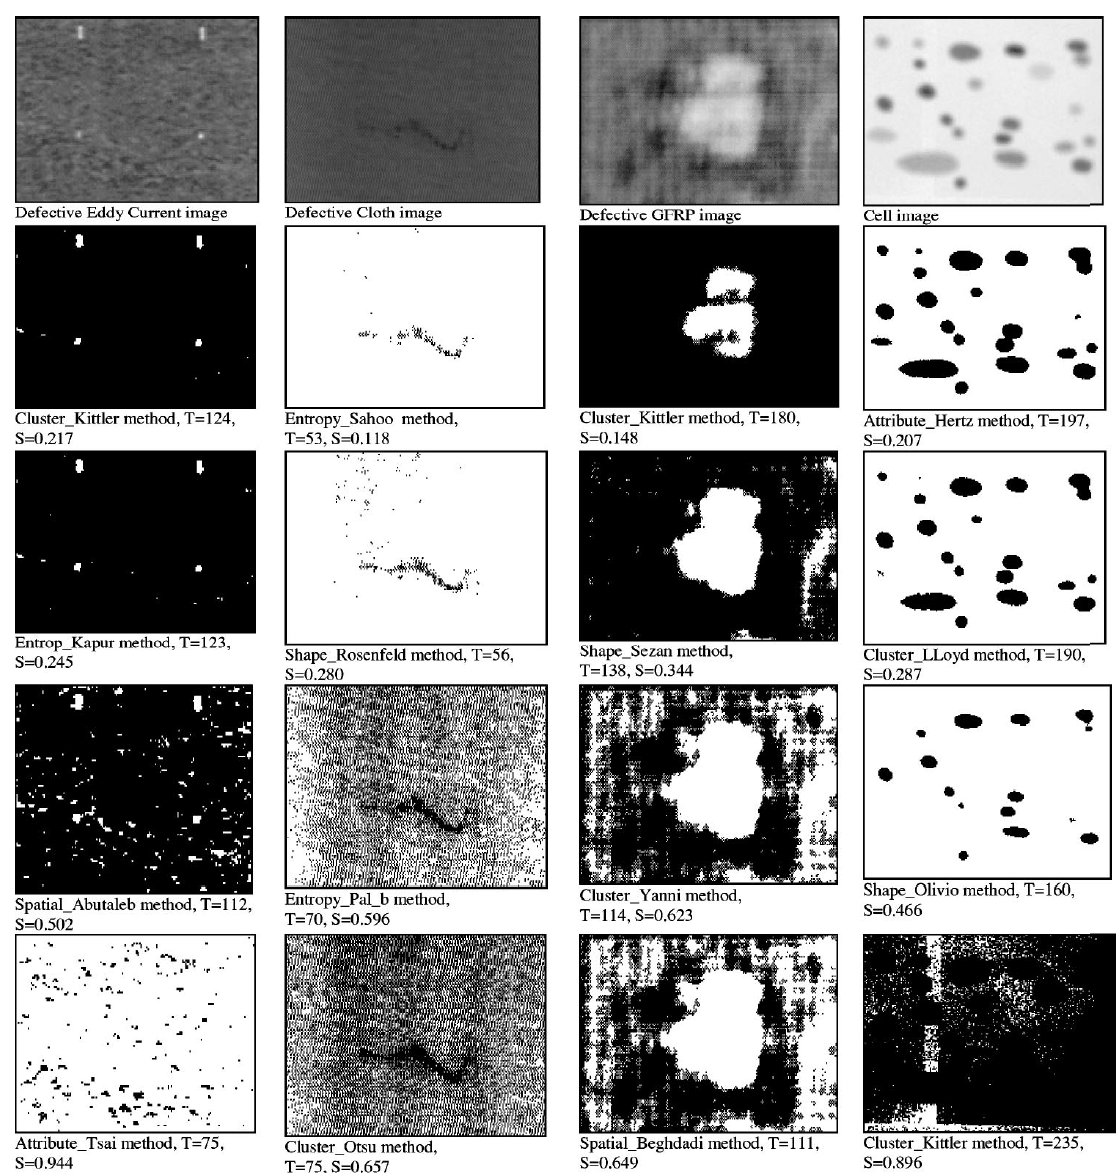
\includegraphics[width=0.9\textwidth,
height=0.6\textwidth]{Figures/fig_threshold_image.png}

\caption[Threshold calculation by different methods]{Different thresholding
results on sample images.\citep{sezgin_survey_2004}}
\label{fig:threshold}
\end{center}

\end{figure}

For our purposes, the binarization threshold will have an impact obtaining the
network. If the threshold is too high, long fibers will break in short,
unconnected pieces. If the threshold is too low, fibers that are clearly
separated, will become blurred together.\\
We have to choose the correct threshold that at the end of the process,
the processed image conserves the topology or architecture of the
original network. The unique way to do that is to rely in the best image
analyser that we have available, our brain . It seems straight forward to choose
the correct binarization threshold despite the initial complexity.
 
\begin{figure}[h]

\begin{minipage}{0.5\textwidth}
\subfloat[Input Image - Original]{%
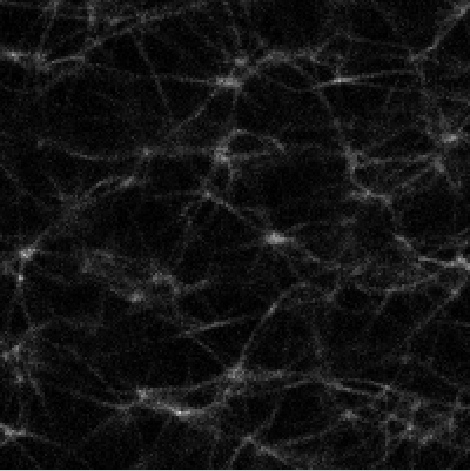
\includegraphics[width=0.9\textwidth]{Figures/binary/fig_bin_original.png}%
\label{original}}
\end{minipage}
\begin{minipage}{0.55\textwidth}
% \begin{minipage}{0.5\textwidth}
\subfloat[$T_P$=0.01]{%
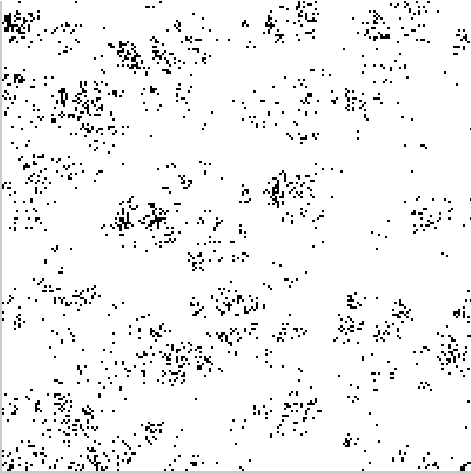
\includegraphics[width=0.45\textwidth]{Figures/binary/fig_bin_01.png}%
\label{001}}
\hspace{1pt}
\subfloat[$T_P$=0.08]{%
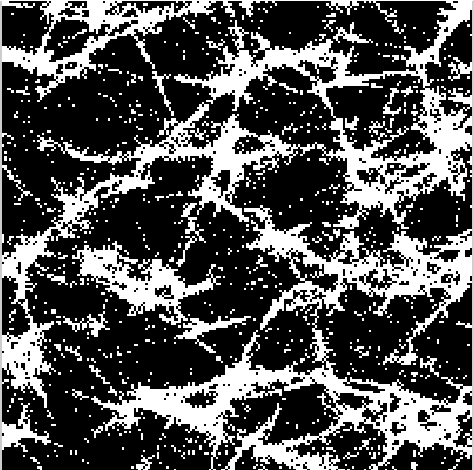
\includegraphics[width=0.45\textwidth]{Figures/binary/fig_bin_08.png}%
\label{008}}

\subfloat[$T_P$=0.1176]{%
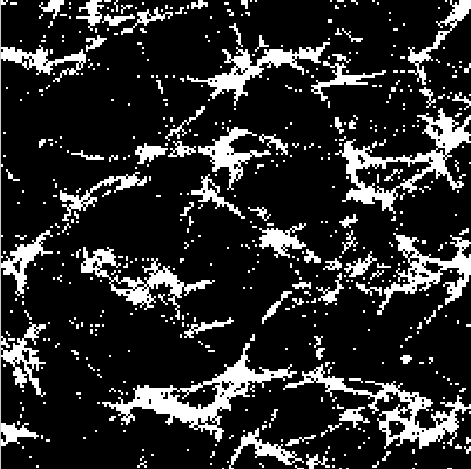
\includegraphics[width=0.45\textwidth]{Figures/binary/fig_bin_01176Otsu.png}%
\label{otsu}}
\hspace{1pt}
\subfloat[$T_P$=0.14]{%
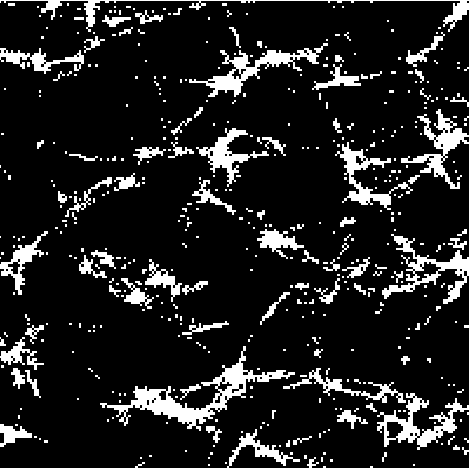
\includegraphics[width=0.45\textwidth]{Figures/binary/fig_bin_14.png}%
\label{014}}
\end{minipage}
% \\
% a)Original Image
% 
% % \end{subfigure}
% \\
% \begin{minipage}{0.5\textwidth}
% 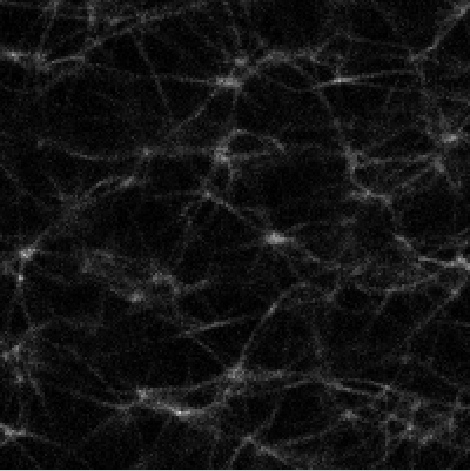
\includegraphics[width=0.3\textwidth]{Figures/binary/fig_bin_original.png}
% 
% \end{minipage}
\caption[Different threshold values on networks]{Different threshold values in
Actin network.
$T_P$ is the threshold value expressed as the percentage of the brightest pixel. If
$P_{max}$ is the brightest pixel, then $T=T_P\cdot P_{max}$. According to eq \ref{eq:bin}, any pixel greater than
that value is $1$ (white) at the output. At low values of threshold we have
blurred networks, at high values, connectivity information is lost.
\subref{otsu} corresponds to the threshold calculated by the Otsu's method }
\label{fig:binary}
\end{figure}

 
\section{FIbeR Extraction -FIRE- algorithm}

 I have used the algorithm from \citep{stein_algorithm_2008}. It is developed to
 analyze confocal stack of images. I have access to it after  Similar procedure.
 Note that in the future I would have to adapt this kind of algorithm to TEM
 tomography image stacks, where the $3D$ resolution might be worse. 
 \begin{description}
 \item[Smooth filter] Smooth the image with a Gaussian filter
 \item[Binarization threshold] Keep a percentage of the brightest pixels
 \item[Distance function- D] gfdgdfg
 
 \subitem \textbf{Smooth filter}
 \item[Nucleation points -NP-]
 \item[Local Maximum Points -LMP-]
 \end{description}
     
This analysis method \citep{stein_algorithm_2008} is based on a original idea of
\citet{wu_automated_2003}. Comparing both
algorithms, \citet{stein_algorithm_2008} main difference is the use of
multiple nucleation points and the restriction that each branch extend only in a single direction from a nucleation
point. In \citet{wu_automated_2003} the network has a single nucleation point 
at the global maximum of the distance function D.


%-----------------------------------
%	SUBSECTION 1
%-----------------------------------
\section{Skeletonization in Avizo}
The Avizo package XSkeleton. The access to Avizo is granted by a collaboration
with from Fonterra.

Step by step
 \begin{description}
 \item[Smooth filter] Smooth the image with a Gaussian filter
 \item[Binarization threshold] Multi-threshold module. This threshold is not
 based in percentage of the brightest pixel. It is a classical threshold turning
 to pure white $255$ or logical $1$ all pixels with a value greatest than the
 threshold value, and black $0$ all the pixels below that value.
 \item[Distance map] Distance map using Euclid distance. It assigns a value
 to each pixel equal to the distance from that pixel to the nearest black value. 
 \item[Thinner module] The module takes as input a label-field to be thinned and
 a distance map scalar field. It removes voxel by voxel from the segmented
 object until only a string of connected voxels remains.
 The thinning algorithm automatically detects dead end branches of skeleton
 spatial graphs. A parameter is used to distinguish them from noise on the
 interface  of the considered regions to avoid spurious branches.  Its default
 value is 5, i.e. the branches with a dead end which length is lower  than 5
 voxels are automatically considered as noise and removed.  Setting this to 10,
 which is a rather large value, leads to only a few branches remaining in the
 skeleton.  The drawback is that you also might miss real endpoints.
 
\item[Tace lines module] Converts an image that contains lines represented by
voxels into a spatial graph object.

 \end{description}

\begin{figure}[h]

% \begin{minipage}{0.5\textwidth}
 
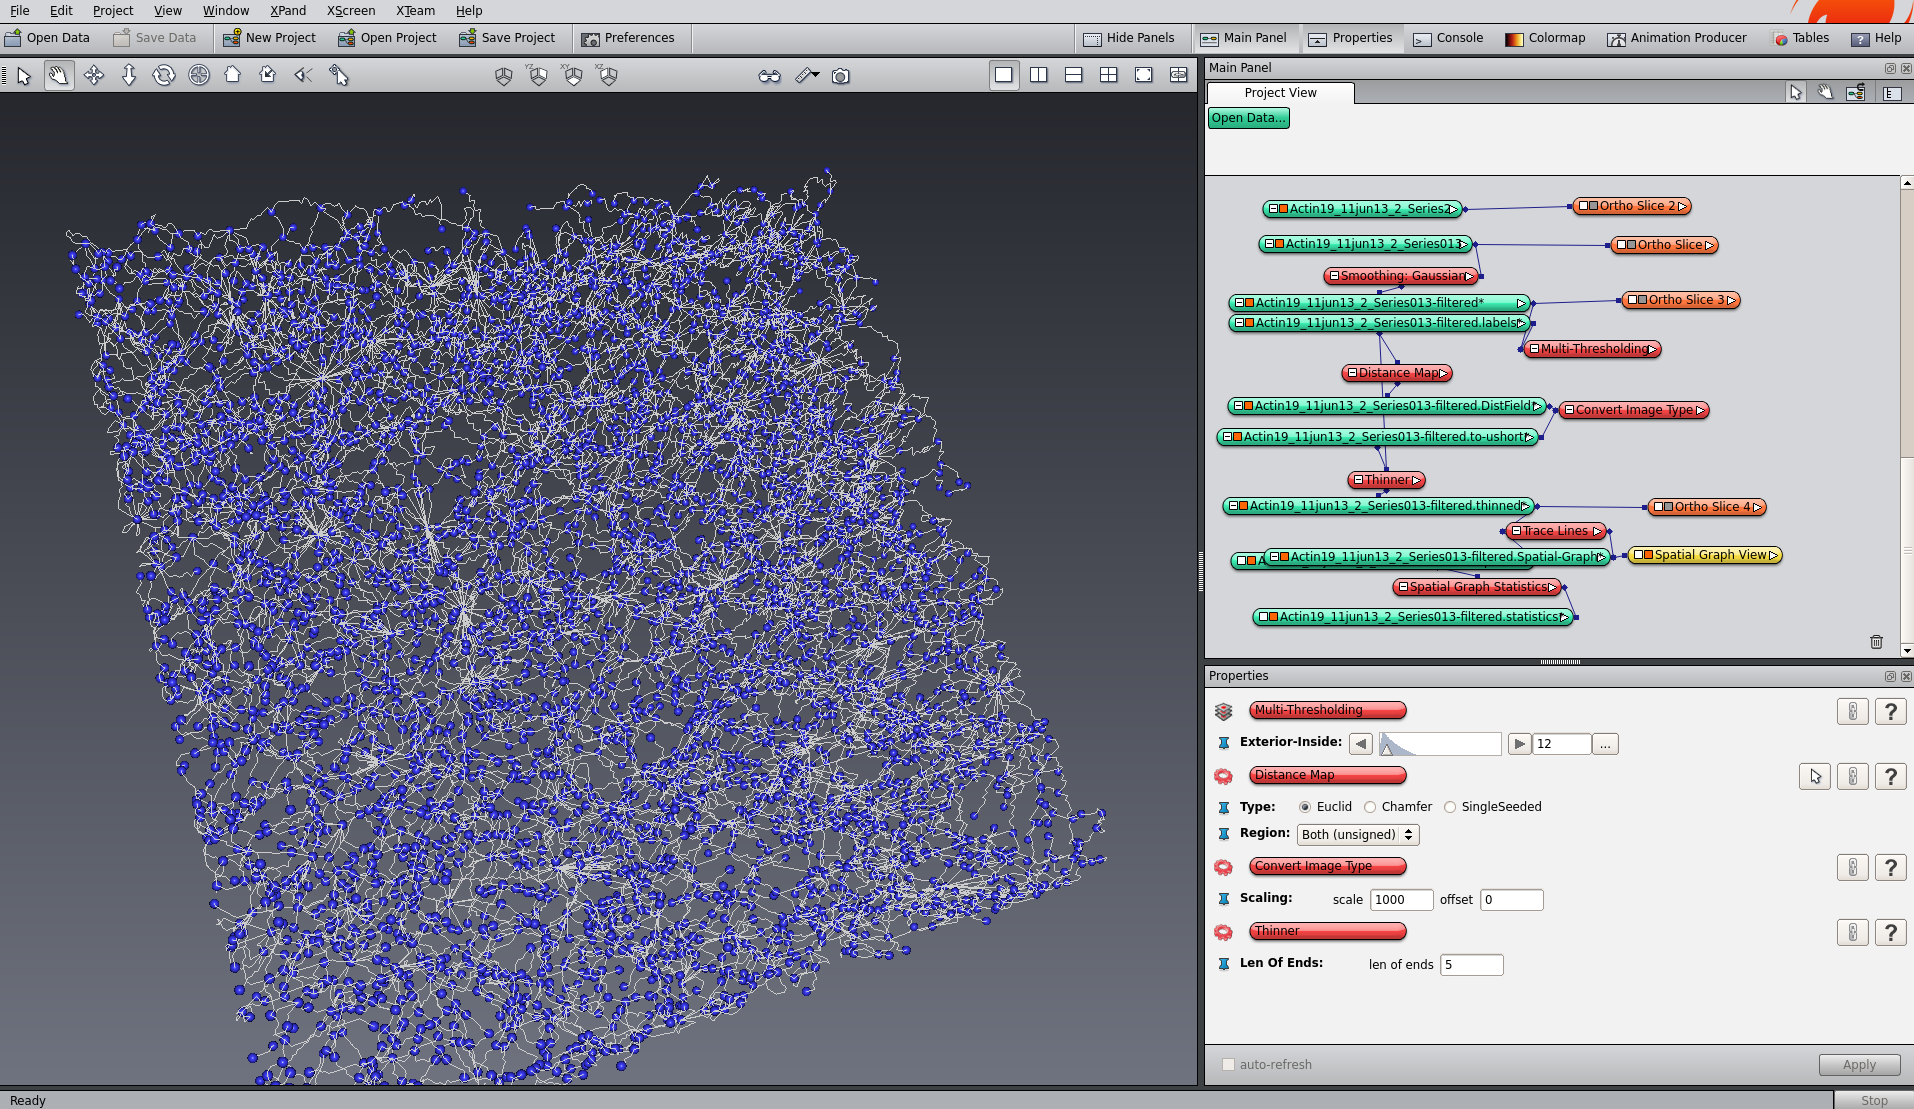
\includegraphics[width=1.1\textwidth]{Figures/avizoworkspaceactin.png}%

% \end{minipage}

% \\
% a)Original Image
% 
% % \end{subfigure}
% \\
% \begin{minipage}{0.5\textwidth}
% 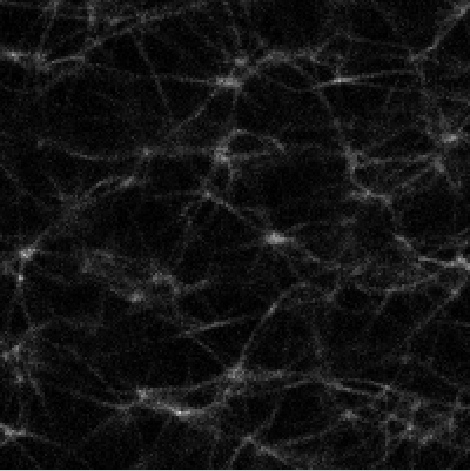
\includegraphics[width=0.3\textwidth]{Figures/binary/fig_bin_original.png}
% 
% \end{minipage}
\caption[Avizo image: Actin network visualization and workspace]{Avizo
workspace. Actin data visualization}
\label{fig:avizo_workspace}
\end{figure}

\section{Results}

Here we use 

 
% Chapter Template

\chapter{Reconstructing networks from statistical distributions} % Main
% chapter title

\label{Chapter-Reconstruction} % Change X to a consecutive number; for
% referencing this chapter elsewhere, use \ref{ChapterX}

\lhead{Chapter 3. \emph{Reconstructing the network from statistical
distributions}} % Change X to a consecutive number; this is for the header on each page - perhaps a shortened title

%----------------------------------------------------------------------------------------
%	SECTION 1
%----------------------------------------------------------------------------------------

\section{Lindstrom Paper}

Lorem ipsum dolor sit amet, consectetur adipiscing elit. Aliquam ultricies lacinia euismod. Nam tempus risus in dolor rhoncus in interdum enim tincidunt. Donec vel nunc neque. In condimentum ullamcorper quam non consequat. Fusce sagittis tempor feugiat. Fusce magna erat, molestie eu convallis ut, tempus sed arcu. Quisque molestie, ante a tincidunt ullamcorper, sapien enim dignissim lacus, in semper nibh erat lobortis purus. Integer dapibus ligula ac risus convallis pellentesque.

%-----------------------------------
%	SUBSECTION 1
%-----------------------------------
\subsection{Subsection 1}

Nunc posuere quam at lectus tristique eu ultrices augue venenatis. Vestibulum ante ipsum primis in faucibus orci luctus et ultrices posuere cubilia Curae; Aliquam erat volutpat. Vivamus sodales tortor eget quam adipiscing in vulputate ante ullamcorper. Sed eros ante, lacinia et sollicitudin et, aliquam sit amet augue. In hac habitasse platea dictumst.

%-----------------------------------
%	SUBSECTION 2
%-----------------------------------

\subsection{Subsection 2}
Morbi rutrum odio eget arcu adipiscing sodales. Aenean et purus a est pulvinar pellentesque. Cras in elit neque, quis varius elit. Phasellus fringilla, nibh eu tempus venenatis, dolor elit posuere quam, quis adipiscing urna leo nec orci. Sed nec nulla auctor odio aliquet consequat. Ut nec nulla in ante ullamcorper aliquam at sed dolor. Phasellus fermentum magna in augue gravida cursus. Cras sed pretium lorem. Pellentesque eget ornare odio. Proin accumsan, massa viverra cursus pharetra, ipsum nisi lobortis velit, a malesuada dolor lorem eu neque.

%----------------------------------------------------------------------------------------
%	SECTION 2
%----------------------------------------------------------------------------------------

\section{Development}

Sed ullamcorper quam eu nisl interdum at interdum enim egestas. Aliquam placerat justo sed lectus lobortis ut porta nisl porttitor. Vestibulum mi dolor, lacinia molestie gravida at, tempus vitae ligula. Donec eget quam sapien, in viverra eros. Donec pellentesque justo a massa fringilla non vestibulum metus vestibulum. Vestibulum in orci quis felis tempor lacinia. Vivamus ornare ultrices facilisis. Ut hendrerit volutpat vulputate. Morbi condimentum venenatis augue, id porta ipsum vulputate in. Curabitur luctus tempus justo. Vestibulum risus lectus, adipiscing nec condimentum quis, condimentum nec nisl. Aliquam dictum sagittis velit sed iaculis. Morbi tristique augue sit amet nulla pulvinar id facilisis ligula mollis. Nam elit libero, tincidunt ut aliquam at, molestie in quam. Aenean rhoncus vehicula hendrerit.
% Chapter Template

\chapter{Schedule and future work} % Main
% chapter title

\label{Chapter-future} % Change X to a consecutive number; for
% referencing this chapter elsewhere, use \ref{ChapterX}

\lhead{Chapter 3. \emph{Schedule and future work}} % Change X to a consecutive
% number; this is for the header on each page - perhaps a shortened title

%----------------------------------------------------------------------------------------
%	SECTION 1
%----------------------------------------------------------------------------------------

\section{Schedule}

\begin{description}
  \item[0-6 months] Landing. Literature overview. Planification and research on
  computational tools.
  \item[6-12 months] Reconstruct-network software development.
   Access to image analysis tools. Avizo and Matlab.
  \item[12-18 months] Selection/development of proper model in order to simulate
  the strain of the network. Think about how simulate long time behavior in the
  networks.
  \item[18-24 months] Explore models and other theoretical frameworks.
  Scaling and renormalization group theory, graph theory to explore strain
  pathways and other networks properties. Plausible experimental experience if
  required.
  \item[24-30 months] Put all together with a solid bottom-up and up-bottom
   approach convergent in the mesoscale. Image analysis of real networks,
   dynamics simulation and in-silico reconstructed networks.
   \item[30-36 months] Conclusions and writing of the
   thesis report.
\end{description}

\subsection{Funding:}
This PhD project is funded by the MacDiarmid and Riddet
institute. 

%-----------------------------------
%	SUBSECTION 1
%-----------------------------------
\section{Future directions and interesting questions}

The field is full of opportunities and in continuous development. The exact
direction to follow will rely on further discussion with my supervisor, and the necessities
of the project from which I am receiving funding. The structure of that project,
and my role on it is clear.

\subsection{``Mesocule'' project}
My PhD fundings come from a project which aim is to explore the hierarchical
structures exhibited by many biomaterials. These structured are organized on
multiple length-scales, with emergent properties not shown by individual
components. The mesoscale, the scale between the bottom and the top of
biomaterials, may be a important source of new knowledge of these biomaterials.

The project is formed by
$3$ professors from Victoria, Canterbury and Massey universities, $2 Post-docs$ and $2 PhD students$. We
have meetings every $6$ months to report advances and to choose new directions.
I will briefly summarize the proposed structure of the project: using optical
tweezers, one of the members is able to  measure force
extension curves of a single biopolymer chain. This expertise can also be  used
to measure protein fibrils that other member of the group can create,  different
properties of the fibril can be tweaked in the grow process to make it
interesting.

Then, having measured the mechanical properties of these engineered
fibrils, and with the network architecture information, gathered after doing
image analysis on microscopy images of the network, we will follow a
bottom-up approach \citep{brown_multiscale_2009,schuster_investigating_2012} to
model and compute the mechanical properties of the whole networks from the single-fibril properties.
Then we will compare those simulated results to
bulk rheology measurements in the macro-scale, done by a fourth member.
Also the developed software about reconstructing network will permit us to 
study how the architecture of the network affect the bulk properties of the material.
 





%-----------------------------------
%	SUBSECTION 2
%-----------------------------------

\subsection{Long time behaviour: network quakes and aging}
There are reports in the literature \citep{kajiya_slow_2013}, and also by group
mates\citep{vincent_micro-rheological_2013}, that at long times the network is affected by sudden
de-correlations that occur over a few tenths of a second. The more
plausible conjecture is that such quakes are associated with the release of
chain constraint due to unbinding of cross-links.  This is reported
experimentally in our group  with micro-rheology DWS techniques in the lab.
Current model of networks as the Glassy WLC model, cannot predict this behaviour.  A computer simulation may shed some light on the topic.

It is also interesting the aging phenomena: the slow change of the physical
properties over time. This behaviour is related with non-ergodic systems and
with glassy systems, where long orders correlations(solids) no longer exists, but there is still local order and
homogeneities.\citep{cipelletti_slow_????}

\subsection{Cluster of nodes as mesoscale objects}
The resolution of image analysis is not enough to provide the network
architecture in some high density areas of the material. These clusters could
then be treated as new mesocule objects, similar to nodes, but with different
properties to those that represent cross-links. This scaling approach could be
study with the renormalization group theory, which has been successful to explain
scaling behavior of polymers in the past.\citep{gennes_scaling_1979}

\subsection{Computational methods}  
The last Nobel prize in Chemistry was given "for the development of multi-scale
models for complex chemical systems" \citep{nobel:chemistry2013} These methods
allow the simulation of protein structures,  docking of drugs in cells and
multiple complex chemical reactions.

These coarse-graining methods study really complex
systems,\citep{de_pablo_coarse-grained_2011} impossible to compute with  the
fine detail potentials of molecular dynamics, but with effective potentials 
derived from scaling, coarse grain and renormalization group theories. These
effective potentials contain the information of the lower scales and can be
tweaked if that information changes, but it is not necessary to simulate all the
degrees of freedom of the fine structure. The communication over scales is the
responsible of the success of the method, where changes in the lower scales are
highly correlated with scales larger by several orders of magnitude. To achieve
this advanced Monte Carlo methods are in continuous development.
\citep{karayiannis_novel_2002}

There are plenty of other methods to explore, FEM, conjugate gradients, and
a plethora of lattice models seem the most popular in the literature. A future
review about these topic will be needed.


% ---------------------------------------------------------------------------------------

% \section{Future work}

 
%\input{Chapters/Chapter6} 
%\input{Chapters/Chapter7} 
% % Chapter 1

\chapter{Chapter Title Here} % Main chapter title

\label{Chapter1} % For referencing the chapter elsewhere, use \ref{Chapter1} 

\lhead{Chapter 1. \emph{Chapter Title Here}} % This is for the header on each page - perhaps a shortened title

%----------------------------------------------------------------------------------------

\section{Welcome and Thank You}
Welcome to this \LaTeX{} Thesis Template, a beautiful and easy to use template for writing a thesis using the \LaTeX{} typesetting system.

If you are writing a thesis (or will be in the future) and its subject is technical or mathematical (though it doesn't have to be), then creating it in \LaTeX{} is highly recommended as a way to make sure you can just get down to the essential writing without having to worry over formatting or wasting time arguing with your word processor.

\LaTeX{} is easily able to professionally typeset documents that run to hundreds or thousands of pages long. With simple mark-up commands, it automatically sets out the table of contents, margins, page headers and footers and keeps the formatting consistent and beautiful. One of its main strengths is the way it can easily typeset mathematics, even \emph{heavy} mathematics. Even if those equations are the most horribly twisted and most difficult mathematical problems that can only be solved on a super-computer, you can at least count on \LaTeX{} to make them look stunning.

%----------------------------------------------------------------------------------------

\section{Learning \LaTeX{}}

\LaTeX{} is not a WYSIWYG (What You See is What You Get) program, unlike word processors such as Microsoft Word or Apple's Pages. Instead, a document written for \LaTeX{} is actually a simple, plain text file that contains \emph{no formatting}. You tell \LaTeX{} how you want the formatting in the finished document by writing in simple commands amongst the text, for example, if I want to use \textit{italic text for emphasis}, I write the `$\backslash$\texttt{textit}\{\}' command and put the text I want in italics in between the curly braces. This means that \LaTeX{} is a ``mark-up'' language, very much like HTML.

\subsection{A (not so short) Introduction to \LaTeX{}}

If you are new to \LaTeX{}, there is a very good eBook -- freely available online as a PDF file -- called, ``The Not So Short Introduction to \LaTeX{}''. The book's title is typically shortened to just ``lshort''. You can download the latest version (as it is occasionally updated) from here:\\
\href{http://www.ctan.org/tex-archive/info/lshort/english/lshort.pdf}{\texttt{http://www.ctan.org/tex-archive/info/lshort/english/lshort.pdf}}

It is also available in several other languages. Find yours from the list on this page:\\
\href{http://www.ctan.org/tex-archive/info/lshort/}{\texttt{http://www.ctan.org/tex-archive/info/lshort/}}

It is recommended to take a little time out to learn how to use \LaTeX{} by creating several, small `test' documents. Making the effort now means you're not stuck learning the system when what you \emph{really} need to be doing is writing your thesis.

\subsection{A Short Math Guide for \LaTeX{}}

If you are writing a technical or mathematical thesis, then you may want to read the document by the AMS (American Mathematical Society) called, ``A Short Math Guide for \LaTeX{}''. It can be found online here:\\
\href{http://www.ams.org/tex/amslatex.html}{\texttt{http://www.ams.org/tex/amslatex.html}}\\
under the ``Additional Documentation'' section towards the bottom of the page.

\subsection{Common \LaTeX{} Math Symbols}
There are a multitude of mathematical symbols available for \LaTeX{} and it would take a great effort to learn the commands for them all. The most common ones you are likely to use are shown on this page:\\
\href{http://www.sunilpatel.co.uk/latexsymbols.html}{\texttt{http://www.sunilpatel.co.uk/latexsymbols.html}}

You can use this page as a reference or crib sheet, the symbols are rendered as large, high quality images so you can quickly find the \LaTeX{} command for the symbol you need.

\subsection{\LaTeX{} on a Mac}
 
The \LaTeX{} package is available for many systems including Windows, Linux and Mac OS X. The package for OS X is called MacTeX and it contains all the applications you need -- bundled together and pre-customised -- for a fully working \LaTeX{} environment and workflow.
 
MacTeX includes a dedicated \LaTeX{} IDE (Integrated Development Environment) called ``TeXShop'' for writing your `\texttt{.tex}' files and ``BibDesk'': a program to manage your references and create your bibliography section just as easily as managing songs and creating playlists in iTunes.

%----------------------------------------------------------------------------------------

\section{Getting Started with this Template}

If you are familiar with \LaTeX{}, then you can familiarise yourself with the contents of the Zip file and the directory structure and then place your own information into the `\texttt{Thesis.cls}' file. Section \ref{FillingFile} on page \pageref{FillingFile} tells you how to do this. Make sure you read section \ref{ThesisConventions} about thesis conventions to get the most out of this template and then get started with the `\texttt{Thesis.tex}' file straightaway.

If you are new to \LaTeX{} it is recommended that you carry on reading through the rest of the information in this document.

\subsection{About this Template}

This \LaTeX{} Thesis Template is originally based and created around a \LaTeX{} style file created by Steve R.\ Gunn from the University of Southampton (UK), department of Electronics and Computer Science. You can find his original thesis style file at his site, here:\\
\href{http://www.ecs.soton.ac.uk/~srg/softwaretools/document/templates/}{\texttt{http://www.ecs.soton.ac.uk/$\sim$srg/softwaretools/document/templates/}}

My thesis originally used the `\texttt{ecsthesis.cls}' from his list of styles. However, I knew \LaTeX{} could still format better. To get the look I wanted, I modified his style and also created a skeleton framework and folder structure to place the thesis files in.

This Thesis Template consists of that modified style, the framework and the folder structure. All the work that has gone into the preparation and groundwork means that all you have to bother about is the writing.

Before you begin using this template you should ensure that its style complies with the thesis style guidelines imposed by your institution. In most cases this template style and layout will be suitable. If it is not, it may only require a small change to bring the template in line with your institution's recommendations.

%----------------------------------------------------------------------------------------

\section{What this Template Includes}

\subsection{Folders}

This template comes as a single Zip file that expands out to many files and folders. The folder names are mostly self-explanatory:

\textbf{Appendices} -- this is the folder where you put the appendices. Each appendix should go into its own separate `\texttt{.tex}' file. A template is included in the directory.

\textbf{Chapters} -- this is the folder where you put the thesis chapters. A thesis usually has about seven chapters, though there is no hard rule on this. Each chapter should go in its own separate `\texttt{.tex}' file and they usually are split as:
\begin{itemize}
\item Chapter 1: Introduction to the thesis topic
\item Chapter 2: Background information and theory
\item Chapter 3: (Laboratory) experimental setup
\item Chapter 4: Details of experiment 1
\item Chapter 5: Details of experiment 2
\item Chapter 6: Discussion of the experimental results
\item Chapter 7: Conclusion and future directions
\end{itemize}
This chapter layout is specialised for the experimental sciences.

\textbf{Figures} -- this folder contains all figures for the thesis. These are the final images that will go into the thesis document.

\textbf{Primitives} -- this is the folder that contains scraps, particularly because one final image in the `Figures' folder may be made from many separate images and photos, these source images go here. This keeps the intermediate files separate from the final thesis figures.

\subsection{Files}

Included are also several files, most of them are plain text and you can see their contents in a text editor. Luckily, many of them are auxiliary files created by \LaTeX{} or BibTeX and which you don't need to bother about:

\textbf{Bibliography.bib} -- this is an important file that contains all the bibliographic information and references that you will be citing in the thesis for use with BibTeX. You can write it manually, but there are reference manager programs available that will create and manage it for you. Bibliographies in \LaTeX{} are a large subject and you may need to read about BibTeX before starting with this.

\textbf{Thesis.cls} -- this is an important file. It is the style file that tells \LaTeX{} how to format the thesis. You will also need to open this file in a text editor and fill in your own information (such as name, department, institution). Luckily, this is not too difficult and is explained in section \ref{FillingFile} on page \pageref{FillingFile}.

\textbf{Thesis.pdf} -- this is your beautifully typeset thesis (in the PDF file format) created by \LaTeX{}.

\textbf{Thesis.tex} -- this is an important file. This is the file that you tell \LaTeX{} to compile to produce your thesis as a PDF file. It contains the framework and constructs that tell \LaTeX{} how to layout the thesis. It is heavily commented so you can read exactly what each line of code does and why it is there. After you put your own information into the `\texttt{Thesis.cls}' file, go to this file and begin filling it in -- you have now started your thesis!

\textbf{vector.sty} -- this is a \LaTeX{} package, it tells \LaTeX{} how to typeset mathematical vectors. Using this package is very easy and you can read the documentation on the site (you just need to look at the `\texttt{vector.pdf}' file):\\
\href{http://www.ctan.org/tex-archive/macros/latex/contrib/vector/}{\texttt{http://www.ctan.org/tex-archive/macros/latex/contrib/vector/}}

\textbf{lstpatch.sty} -- this is a \LaTeX{} package required by this LaTeX template and is included as not all \TeX{} distributions have it installed by default. You do not need to modify this file.

Files that are \emph{not} included, but are created by \LaTeX{} as auxiliary files include:

\textbf{Thesis.aux} -- this is an auxiliary file generated by \LaTeX{}, if it is deleted \LaTeX{} simply regenerates it when you run the main `\texttt{.tex}' file.

\textbf{Thesis.bbl} -- this is an auxiliary file generated by BibTeX, if it is deleted, BibTeX simply regenerates it when you run the main tex file. Whereas the `\texttt{.bib}' file contains all the references you have, this `\texttt{.bbl}' file contains the references you have actually cited in the thesis and is used to build the bibliography section of the thesis.

\textbf{Thesis.blg} -- this is an auxiliary file generated by BibTeX, if it is deleted BibTeX simply regenerates it when you run the main `\texttt{.tex}' file.

\textbf{Thesis.lof} -- this is an auxiliary file generated by \LaTeX{}, if it is deleted \LaTeX{} simply regenerates it when you run the main `\texttt{.tex}' file. It tells \LaTeX{} how to build the `List of Figures' section.

\textbf{Thesis.log} -- this is an auxiliary file generated by \LaTeX{}, if it is deleted \LaTeX{} simply regenerates it when you run the main `\texttt{.tex}' file. It contains messages from \LaTeX{}, if you receive errors and warnings from \LaTeX{}, they will be in this `\texttt{.log}' file.

\textbf{Thesis.lot} -- this is an auxiliary file generated by \LaTeX{}, if it is deleted \LaTeX{} simply regenerates it when you run the main `\texttt{.tex}' file. It tells \LaTeX{} how to build the `List of Tables' section.

\textbf{Thesis.out} -- this is an auxiliary file generated by \LaTeX{}, if it is deleted \LaTeX{} simply regenerates it when you run the main `\texttt{.tex}' file.


So from this long list, only the files with the `\texttt{.sty}', `\texttt{.bib}', `\texttt{.cls}' and `\texttt{.tex}' extensions are the most important ones. The other auxiliary files can be ignored or deleted as \LaTeX{} and BibTeX will regenerate them.

%----------------------------------------------------------------------------------------

\section{Filling in the `\texttt{Thesis.cls}' File}\label{FillingFile}

You will need to personalise the thesis template and make it your own by filling in your own information. This is done by editing the `\texttt{Thesis.cls}' file in a text editor.

Open the file and scroll down, past all the `$\backslash$\texttt{newcommand}\ldots' items until you see the entries for `\texttt{University Name}', `\texttt{Department Name}', etc\ldots.

Fill out the information about your group and institution and ensure you keep to block capitals where it asks you to. You can also insert web links, if you do, make sure you use the full URL, including the `\texttt{http://}' for this.

The last item you should need to fill in is the Faculty Name (in block capitals). When you have done this, save the file and recompile `\texttt{Thesis.tex}'. All the information you filled in should now be in the PDF, complete with web links. You can now begin your thesis proper!

%----------------------------------------------------------------------------------------

\section{The `\texttt{Thesis.tex}' File Explained}

The \texttt{Thesis.tex} file contains the structure of the thesis. There are plenty of written comments that explain what pages, sections and formatting the \LaTeX{} code is creating. Initially there seems to be a lot of \LaTeX{} code, but this is all formatting, and it has all been taken care of so you don't have to do it.

Begin by checking that your information on the title page is correct. For the thesis declaration, your institution may insist on something different than the text given. If this is the case, just replace what you see with what is required.

Then comes a page which contains a funny quote. You can put your own, or quote your favourite scientist, author, person, etc\ldots Make sure to put the name of the person who you took the quote from.

Next comes the acknowledgements. On this page, write about all the people who you wish to thank (not forgetting parents, partners and your advisor/supervisor).

The contents pages, list of figures and tables are all taken care of for you and do not need to be manually created or edited. The next set of pages are optional and can be deleted since they are for a more technical thesis: insert a list of abbreviations you have used in the thesis, then a list of the physical constants and numbers you refer to and finally, a list of mathematical symbols used in any formulae. Making the effort to fill these tables means the reader has a one-stop place to refer to instead of searching the internet and references to try and find out what you meant by certain abbreviations or symbols.

The list of symbols is split into the Roman and Greek alphabets. Whereas the abbreviations and symbols ought to be listed in alphabetical order (and this is \emph{not} done automatically for you) the list of physical constants should be grouped into similar themes.

The next page contains a one line dedication. Who will you dedicate your thesis to?

Finally, there is the section where the chapters are included. Uncomment the lines (delete the `\texttt{\%}' character) as you write the chapters. Each chapter should be written in its own file and put into the `Chapters' folder and named `\texttt{Chapter1}', `\texttt{Chapter2}, etc\ldots Similarly for the appendices, uncomment the lines as you need them. Each appendix should go into its own file and placed in the `Appendices' folder.

After the preamble, chapters and appendices finally comes the bibliography. The bibliography style (called `\texttt{unsrtnat}') is used for the bibliography and is a fully featured style that will even include links to where the referenced paper can be found online. Do not under estimate how grateful you reader will be to find that a reference to a paper is just a click away. Of course, this relies on you putting the URL information into the BibTeX file in the first place.

%----------------------------------------------------------------------------------------

\section{Thesis Features and Conventions}\label{ThesisConventions}

To get the best out of this template, there are a few conventions that you may want to follow.

One of the most important (and most difficult) things to keep track of in such a long document as a thesis is consistency. Using certain conventions and ways of doing things (such as using a Todo list) makes the job easier. Of course, all of these are optional and you can adopt your own method.

\subsection{Printing Format}

This thesis template is designed for single sided printing as most theses are printed and bound this way. This means that the left margin is always wider than the right (for binding). Four out of five people will now judge the margins by eye and think, ``I never 
noticed that before.''.

The headers for the pages contain the page number on the right side (so it is easy to flick through to the page you want) and the chapter name on the left side.

The text is set to 11 point and a line spacing of 1.3. Generally, it is much more readable to have a smaller text size and wider gap between the lines than it is to have a larger text size and smaller gap. Again, you can tune the text size and spacing should you want or need to. The text size can be set in the options for the `$\backslash$\texttt{documentclass}' command at the top of the `\texttt{Thesis.tex}' file and the spacing can be changed by setting a different value in the `$\backslash$\texttt{setstretch}' commands (scattered throughout the `\texttt{Thesis.tex}' file).

\subsection{Using US Letter Paper}

The paper size used in the template is A4, which is a common -- if not standard -- size in Europe. If you are using this thesis template elsewhere and particularly in the United States, then you may have to change the A4 paper size to the US Letter size. Unfortunately, this is not as simple as replacing instances of `\texttt{a4paper}' with `\texttt{letterpaper}'.

This is because the final PDF file is created directly from the \LaTeX{} source using a program called `\texttt{pdfTeX}' and in certain conditions, paper size commands are ignored and all documents are created with the paper size set to the size stated in the configuration file for pdfTeX (called `\texttt{pdftex.cfg}').

What needs to be done is to change the paper size in the configuration file for \texttt{pdfTeX} to reflect the letter size. There is an excellent tutorial on how to do this here: \\
\href{http://www.physics.wm.edu/~norman/latexhints/pdf_papersize.html}{\texttt{http://www.physics.wm.edu/$\sim$norman/latexhints/pdf\_papersize.html}}

It may be sufficient just to replace the dimensions of the A4 paper size with the US Letter size in the \texttt{pdftex.cfg} file. Due to the differences in the paper size, the resulting margins may be different to what you like or require (as it is common for Institutions to dictate certain margin sizes). If this is the case, then the margin sizes can be tweaked by opening up the \texttt{Thesis.cls} file and searching for the line beginning with, `$\backslash$\texttt{setmarginsrb}' (not very far down from the top), there you will see the margins specified. Simply change those values to what you need (or what looks good) and save. Now your document should be set up for US Letter paper size with suitable margins.

\subsection{References}

The `\texttt{natbib}' package is used to format the bibliography and inserts references such as this one \citep{Reference3}. The options used in the `\texttt{Thesis.tex}' file mean that the references are listed in numerical order as they appear in the text. Multiple references are rearranged in numerical order (e.g. \citep{Reference2, Reference1}) and multiple, sequential references become reformatted to a reference range (e.g. \citep{Reference2, Reference1, Reference3}). This is done automatically for you. To see how you use references, have a look at the `\texttt{Chapter1.tex}' source file. Many reference managers allow you to simply drag the reference into the document as you type.

Scientific references should come \emph{before} the punctuation mark if there is one (such as a comma or period). The same goes for footnotes\footnote{Such as this footnote, here down at the bottom of the page.}. You can change this but the most important thing is to keep the convention consistent throughout the thesis. Footnotes themselves should be full, descriptive sentences (beginning with a capital letter and ending with a full stop).

To see how \LaTeX{} typesets the bibliography, have a look at the very end of this document (or just click on the reference number links).

\subsection{Figures}

There will hopefully be many figures in your thesis (that should be placed in the `Figures' folder). The way to insert figures into your thesis is to use a code template like this:
\begin{verbatim}
\begin{figure}[htbp]
  \centering
    
\includegraphics{Figures/Electron.pdf}
    \rule{35em}{0.5pt}
  \caption[An Electron]{An electron (artist's impression).}
  \label{fig:Electron}
\end{figure}
\end{verbatim}
Also look in the source file. Putting this code into the source file produces the picture of the electron that you can see in the figure below.

\begin{figure}[htbp]
	\centering
		
\includegraphics{Figures/Electron.pdf}
		\rule{35em}{0.5pt}
	\caption[An Electron]{An electron (artist's impression).}
	\label{fig:Electron}
\end{figure}

Sometimes figures don't always appear where you write them in the source. The placement depends on how much space there is on the page for the figure. Sometimes there is not enough room to fit a figure directly where it should go (in relation to the text) and so \LaTeX{} puts it at the top of the next page. Positioning figures is the job of \LaTeX{} and so you should only worry about making them look good!

Figures usually should have labels just in case you need to refer to them (such as in Figure \ref{fig:Electron}). The `$\backslash$\texttt{caption}' command contains two parts, the first part, inside the square brackets is the title that will appear in the `List of Figures', and so should be short. The second part in the curly brackets should contain the longer and more descriptive caption text.

The `$\backslash$\texttt{rule}' command is optional and simply puts an aesthetic horizontal line below the image. If you do this for one image, do it for all of them.

The \LaTeX{} Thesis Template is able to use figures that are either in the PDF or JPEG file format.

\subsection{Typesetting mathematics}

If your thesis is going to contain heavy mathematical content, be sure that \LaTeX{} will make it look beautiful, even though it won't be able to solve the equations for you.

The ``Not So Short Introduction to \LaTeX{}'' (available \href{http://www.ctan.org/tex-archive/info/lshort/english/lshort.pdf}{here}) should tell you everything you need to know for most cases of typesetting mathematics. If you need more information, a much more thorough mathematical guide is available from the AMS called, ``A Short Math Guide to \LaTeX{}'' and can be downloaded from:\\
\href{ftp://ftp.ams.org/pub/tex/doc/amsmath/short-math-guide.pdf}{\texttt{ftp://ftp.ams.org/pub/tex/doc/amsmath/short-math-guide.pdf}}

There are many different \LaTeX{} symbols to remember, luckily you can find the most common symbols \href{http://www.sunilpatel.co.uk/latexsymbols.html}{here}. You can use the web page as a quick reference or crib sheet and because the symbols are grouped and rendered as high quality images (each with a downloadable PDF), finding the symbol you need is quick and easy.

You can write an equation, which is automatically given an equation number by \LaTeX{} like this:
\begin{verbatim}
\begin{equation}
E = mc^{2}
  \label{eqn:Einstein}
\end{equation}
\end{verbatim}

This will produce Einstein's famous energy-matter equivalence equation:
\begin{equation}
E = mc^{2}
\label{eqn:Einstein}
\end{equation}

All equations you write (which are not in the middle of paragraph text) are automatically given equation numbers by \LaTeX{}. If you don't want a particular equation numbered, just put the command, `$\backslash$\texttt{nonumber}' immediately after the equation.

%----------------------------------------------------------------------------------------

\section{Sectioning and Subsectioning}

You should break your thesis up into nice, bite-sized sections and subsections. \LaTeX{} automatically builds a table of Contents by looking at all the `$\backslash$\texttt{chapter}$\{\}$', `$\backslash$\texttt{section}$\{\}$' and `$\backslash$\texttt{subsection}$\{\}$' commands you write in the source.

The table of Contents should only list the sections to three (3) levels. A `$\backslash$\texttt{chapter}$\{\}$' is level one (1). A `$\backslash$\texttt{section}$\{\}$' is level two (2) and so a `$\backslash$\texttt{subsection}$\{\}$' is level three (3). In your thesis it is likely that you will even use a `$\backslash$\texttt{subsubsection}$\{\}$', which is level four (4). Adding all these will create an unnecessarily cluttered table of Contents and so you should use the `$\backslash$\texttt{subsubsection$^{*}\{\}$}' command instead (note the asterisk). The asterisk ($^{*}$) tells \LaTeX{} to omit listing the subsubsection in the Contents, keeping it clean and tidy.

%----------------------------------------------------------------------------------------

\section{In Closing}

You have reached the end of this mini-guide. You can now rename or overwrite this pdf file and begin writing your own `\texttt{Chapter1.tex}' and the rest of your thesis. The easy work of setting up the structure and framework has been taken care of for you. It's now your job to fill it out!

Good luck and have lots of fun!

\begin{flushright}
Guide written by ---\\
Sunil Patel: \href{http://www.sunilpatel.co.uk}{www.sunilpatel.co.uk}
\end{flushright}
  
%----------------------------------------------------------------------------------------
%	THESIS CONTENT - APPENDICES
%----------------------------------------------------------------------------------------
   
\addtocontents{toc}{\vspace{2em}} % Add a gap in the Contents, for aesthetics
 
\appendix % Cue to tell LaTeX that the following 'chapters' are Appendices
 
% Include the appendices of the thesis as separate files from the Appendices folder
% Uncomment the lines as you write the Appendices
      
% Appendix A

\chapter{Acquired tools} % Main appendix title

\label{Appendix-tools} % For referencing this appendix elsewhere, use
% \ref{AppendixA}

\lhead{Acquired tools} % This is for the header on each page -
% perhaps a shortened title

\section{Coding : C++}
At the beginning of my PhD, I was not sure about what language to choose for the
development of tools to compute in-silico polymer networks. I had previous
experience with Fortran and Python, but each of them has some drawbacks, and I wanted to start
the project with the most sharp tools available. From my point of
view, the more important characteristics of a language are three :
\begin{enumerate*}[label=\bfseries\alph*)]
\item Fast computation. 
\item Community support and development tools.
\item Learning curve.
\end{enumerate*}
 
Fortran is really fast, its vector/matrix multiplication is unbeatable. The main
drawback of Fortran is that is hard to develop complex projects on it(it easy
to end with a unstructured/messy code), no Object Oriented Programming (OOP)
support and also it has no use at all in any other field different from hardcore numerical computing. Also the community is
tiny, and the language lacks of some really useful libraries.
Even though it is still used in many big projects, sometimes because the project has inherited old code,
 or sometimes because the Fortran speed is needed. 

Python has a huge community, it is a pretty modern language, easy development,
OOP support, widely used in a lot of fields. Programming in Python is kind of a
pleasure because it is closer to the regular way of thinking than any other
language. The unique drawback is that it is really slow, by orders of magnitude
in comparison to Fortran or C++. 

So, I chose to learn C++. I have access to tons of libraries (I am using
Boost Graph Library -to generate the spatial graph-, and Igraph -complex
networks- in my Reconstruct-Network software), it is also the language of $3D$  computing
graphics, in case I want to visualize the networks at fast speed.  It is almost
as fast as Fortran (even faster in some points thanks to the continuous
development of compilers). The drawback of C++ is that is hard to enter and
start learning, but with help of
\href{http://www.stackoverflow.com}{StackOverflow},
\citet{stroustrup_c++_2013}, and \citet{lippman_c++_2013}, I have developed the
Reconstruct-Network software (Chapter \ref{Chapter-Reconstruction}),
and I think I have gained enough expertise in C++ to face future challenges in this project.

\emph{``Premature optimization is the root of all evil.'' Donald Knuth}
\section{Linux environment}

I have gained expertise on Linux
platform, the open source community, and also with some useful software that I
use daily.
 
 \begin{itemize}
   \item Eclipse IDE. Graphic interface for different languages. I have used
   it to work with C++, Python, and this latex manuscript.
   \item Git. Version control software. Software to keep controlled all
   changes in the software under development. Version control is vital to handle
   complex software, and really useful to explore,add or remove modules  with no
   risk of mess it up all previous work. It is also fundamental in collaboration
   projects with other programmers. \href{https://github.com/}{GitHub} is really the hub
   of amazing open source projects created and maintained from the open source community.
   \item Cmake. Multiplatform assistant for managing the build process of
   software. It is required for using computer graphic software, such VTK.
   \item \href{http://www.zotero.org/}{Zotero}. It is a multiplatform open
   source tool for bibliography management (alternative to EndNote, or
   Mendelev).It can be used as an add-on to any internet browser (Firefox -open source- is recommended), and also has a 
   stand-alone version.
 

 \end{itemize}
 






% Appendix Template

\chapter{Software: Reconstruct-Network} % Main appendix title

\label{Appendix-Reconstruct} % Change X to a consecutive letter; for referencing
% this appendix elsewhere, use \ref{AppendixX}

\lhead{Appendix \emph{Reconstruct-Network}} % Change X to a
% consecutive letter; this is for the header on each page - perhaps a shortened title

The  software is based, but independently developed,  on the idea of
\citet{lindstrom_biopolymer_2010} about reconstructing the network
architecture of polymers networks from a statistical description. They were
based on \citet{yeong_reconstructing_1998,yeong_reconstructing_1998-1} work
about  reconstructing random porosity media.\\
The input for the reconstruction is the
statistical distributions of $3$ properties in this case. This is the minimal 
set to reconstruct the correct architecture of the network to study the
mechanical properties, but other parameters could be added to study other or
more complex situations.  For example, if the structure of the edges / chains is
heterogeneous  (bio-functional areas, or different charge distribution), extra
statistical distributions can be added with minimal effort.
\begin{enumerate} 
\item \emph{N}. Degree of nodes. i.e. number of edges per node or cross-link. 
\item \emph{$\ell$}. Length of edges. Length of the edges between connected
% nodes.
There are two options to define this length.
\begin{itemize}
\item End to end vector distance (EtE-length). Consider the edge as a straight
line between nodes.

\item Contour length (curved). Take into account all the path of the chain,
usually curved.
\end{itemize}

The difference between both is lesser that one
might have expected at a first glance. \citet{nisslert_identification_2007},
who use a different reconstructing algorithm, report that straight and curved
lengths have similar distribution, although the straight lines were about a
$15\%$ shorter.\\
I expect that high flexibility of the chains and/or low density of cross-links
will increase the differences between them. Biopolymer are semi-flexible, stiff
enough to keep this difference low.
In any case, if both cases are following the same distribution is just a matter
of scaling the length parameters.\\
The difference between these lengths can be used as a measure of the
persistence length (\gls{Lp}) of the chains.
  

\item \emph{$\beta$}. Cosine director between incident edges. Take into account
the relative orientation of the edges incident to a node.


\end{enumerate}

These parameters can be obtained using \textbf{image analysis} of data from
\gls{confocal}, transmission electron microscopy (\gls{TEM}) or
scanning electron microscopy \gls{SEM}. See chapter \ref{Chapter-Image} for
more information about this process.

The follow distributions are used because they fit the data taken from image
analysis, but I make no claim about their use in other systems. The
direction cosines distribution has a lot of variability. I have experienced
these differences between actin and collagen data.
\begin{enumerate} 
\item The node degrees follow a shifted geometric distribution. Shifted because
the minimum degree of a node is $p=3$.$p=1$ corresponds to dead-ends nodes, and
$p=2$ correspond to bending nodes. We can ignore dead-ends because they don't
affect to the mechanical properties of the bulk network. And the bending nodes
can be ignored if its $2$ edges are merged into a unique, larger edge,
connecting the neighbors of this bending node between them. Some information is lost in this
process if we are characterizing the length of edges by end to end
vectors.
\begin{equation} \label{degree-dist}
N(p)=q(1-q)^{p-3} 
\end{equation}
where $q=1/(Z-2)$ , and Z is the average node degree.
\item The length distribution is logarithmic-normal  
\begin{equation} \label{length-dist}
P(\ell)=\frac{1}{\ell
s\sqrt{2\pi}}\exp{\bigg[-\frac{(\mu-\ln{\ell})^2}{2s^2}\bigg]}
\end{equation}
where $\mu$ and s are the mean and standard deviation of $\ln{\ell}$
respectively.
%CHECK THAT LINDSTROM SAYS THAT \ell is normalized by n^{-1/3}
\item The director cosines distribution can be represented by a truncated power
series.
\begin{equation} \label{cosines-dist}
B(\beta)=\sum_{k=1}^{m} b_k(1-\beta)^{2k-1}
\end{equation}
If we truncate it at $m=3$, and $B(\beta)$ is normalized to unity, then there
are two parameters left, $b_1$ and $b_2$ (or other combination).
\end{enumerate}

Using these $3$ distributions, the network can be reconstructed with five
independent parameters: $\mu$, s, $Z$, $b_1$ and $b_2$.

These parameters are enough to fully characterize the architecture of a
network if you are interested in computing the
mechanical properties of the system.

The output of the algorithm is spatial \gls{graph}, which is formed by $2$
sets. The first set is associated with the nodes, and contains the data of node
position and degree. The second set is a list of edges, an edge is defined
by two nodes which the edge is connecting. The software does not allow parallel
edges, i.e. two edges connected the same pair of nodes, and the network is fully
connected, there are no nodes or clusters of nodes isolated from the rest of the
network.
 
 
 
% % Appendix doxygen


\chapter{Software documentation: Doxygen} % Main appendix
% title

\pagestyle{empty} 
\label{AppendixDoxygen} % For referencing this appendix elsewhere, use
% \ref{AppendixA}

\lhead{Appendix \emph{Software documentation}} % This is for the header on each
% page - perhaps a shortened title

%break the links, maybe you should the numbering to \pagenumbering{non-arabic}
% in the generated refman.tex, and then pdflatex that.
\includepdf[delta=0mm 0mm,
offset=20mm 0mm
,pages=-]{/home/phc/workspace/EGG/Documentation/latex/refman.pdf}
%   nup=2x2,,templatesize={4cm}{4cm}


 
%\input{Appendices/AppendixC}

%%%%%%%%%%%%%%%%GLOSSARY ENTRIES%%%%%%%%%%%%%%%%%%%%%%%%
\clearpage
\setstretch{1.5} % Set the line spacing to 1.5, this makes the following tables easier to read
 
\lhead{\emph{Glossary}} % Set the left side page header to "Abbreviations"


\addcontentsline{toc}{chapter}{Glossary}
\glsaddall 
\printglossaries 

%%%%%%%%%%%%%%%%%%%%%%%%%%%%%%%%%%%%%%%%%%%%%%%%%%%%%%%%%




\addtocontents{toc}{\vspace{2em}} % Add a gap in the Contents, for aesthetics

\backmatter
   
%----------------------------------------------------------------------------------------
%	BIBLIOGRAPHY
%----------------------------------------------------------------------------------------
 
\label{References}

\lhead{\emph{References}} % Change the page header to say "Bibliography"

\bibliographystyle{unsrtnat} % Use the "unsrtnat" BibTeX style for formatting the Bibliography

\bibliography{MyLibrary} % The references (bibliography) information are stored
% in the file named "Bibliography.bib"
%----------------------------------------------------------------------------------------
%	GLOSSARY
%----------------------------------------------------------------------------------------
 

\end{document}  